\chapter{Background: USB Devices}
\label{chap:rel_work}
In the early days of computers, various connectors existed for computers to communicate with external devices. A few examples of such connectors are the PS/2 port (Primarily used for Mouse / Keyboard) or the Parallel port (Often used for printers). These connectors have varying sizes, shapes and limitations and cannot be used for all devices. Therefore, computers needed to have all these ports, requiring lots of space. To address these issues, the USB connector was introduced. Years later, the interface has become the de-facto standard for wired device communication. Over the years, USB has evolved with multiple revisions. These revisions focus on key aspects of the interface, such as transfer speeds, power delivery and added functionality. The USB connector has also undergone revisions, making it smaller and reversible, so it is usable on a larger variety of devices.

In this thesis, the focus is on the software side of the USB standard. Therefore, the hardware will not be considered further.

\section{Transferring Data via USB}

This is an introduction of the internals of the USB protocol. For more information, take a look at \href{https://www.beyondlogic.org/usbnutshell/usb1.shtml}{USB in a NutShell}
\subsection{Pipes}
Data is transferred through pipes. A pipe is a connection from the host controller to the endpoint. Not all pipes are the same: they differ in the bandwidth they support, which transfer types are supported, in which direction data can flow, and their packet and buffer size. Pipes can generally be split up into two kinds.

\subsubsection{Streaming Pipes}
A Streaming Pipe is a one-way communication channel for the host or guest device to send any kind of data to the other end. This pipe is controlled by either the host of or guest device, and data is sent in a sequential way. The isochronous, interrupt and bulk transfer types will use this pipe to send data.

\subsubsection{Message Pipes}
A Message Pipe is a bidirectional communication channel. This pipe allows both the host and guest device to send commands in either direction on the same pipe. All message pipes are controlled by the host device. Only one transfer type supports this pipe: the control transfer type.

\subsection{Transfer Types}
\label{section:transfer_types}
The USB standard defines four transfer types. Each transfer type serves a different purpose, being optimized for speed, latency, correctness or reliability.

\subsubsection{Interrupt Transfer}
Interrupt transfers are most used for devices that transfer small amounts of data frequently. They have a bounded latency and are therefore suited for devices that require low latency and low bandwidth. Interrupt transfers can be initiated by both the host and guest device. The sent data will be queued by the sender, until the receiver polls the device.

Examples of devices that often use interrupt transfers are mice and keyboards.

\subsubsection{Isochronous Transfer}
Isochronous transfers are used for real-time data streaming. They provide a guaranteed data rate, but do not guarantee a correct transfer of data, and data can be lost. This makes the transfer type not suitable for situations where data integrity is important.

Examples of use cases where isochronous data transfer is often used is for audio devices or video streaming.

\subsubsection{Bulk Transfer}
Bulk transfers are suited for transferring large amounts of data where timing is not an issue, but data integrity is. No guarantee on timing is made, but guaranteed correct delivery is.

Examples of use cases for bulk transfers are sending files to printers or storage devices.

\subsubsection{Control Transfer}
Control transfers are used for configuration, command and status operations between the host and guest device. Control transfers operate on the Message pipe and has setup, data and handshake stages. The handshakes guarantee correct delivery, but will lead to a slower transfer speed. Therefore, control transfers are not used to transfer a lot of data, but rather for device initialization and control.

The Control transfer type can be seen as a TCP connection but for USB devices.

\subsection{Descriptors}

Descriptors are used numerous times throughout the USB specification. They define a standardized way to provide information about a part of the specification.

Details of each descriptor can be found in the appendix \ref{appendix:descriptors}.

\begin{figure}[h]
  \centering
  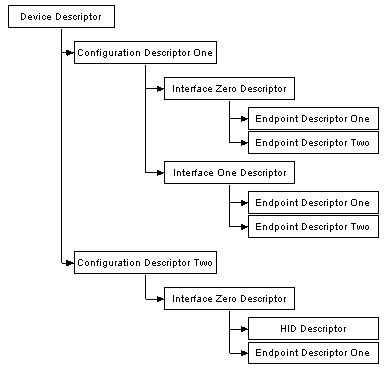
\includegraphics[width=0.5\textwidth]{images/descriptor_tree.png}
  \caption{Descriptor Tree of a USB device. This tree contains all useful metadata to communicate with the device.}
  \label{fig:descriptor_tree}
\end{figure}

\subsubsection{Device Descriptors}

Each USB device has a device descriptor, which contains general information about the device, such as what name is has, which protocols it supports, its serial number, how much configurations it has, and more. This descriptor is essentially the entrypoint to do anything with the device.

\subsubsection{Configuration Descriptors}

The configuration descriptor provides information about a configuration of a USB device. A devices can have multiple configurations, each defining different combinations of interfaces and endpoints that the device supports.

Each configuration descriptor contains a standardized set of fields, such as how many interfaces it contains (and the descriptors for these interfaces), or the power consumption of the configuration. The host device can also determine if the device is self-powered or bus-powered based off the configuration descriptor.

When a USB device is connected to a host, the host uses the configuration descriptor to determine which configuration to activate and how to communicate with the device.

\subsubsection{Interface Descriptors}

The interface descriptor provides information such as the interface number, the alternate setting number (if multiple settings are available for the interface), the number of endpoints associated with the interface, and more.

\subsubsection{Endpoint Descriptors}

Endpoints are the communication channels through which data is transmitted between the host device and the USB device.

The endpoint descriptor provides information such as the endpoint address (with the direction of data flow), transfer speed, transfer type (see \ref{section:transfer_types}), and more.

Each endpoint can have any transfer type, except for endpoint zero. This endpoint is assumed to be a control endpoint, and will have a control transfer type. Endpoint zero will be used to communicate with the device to get its descriptors.

\section{Existing Solutions}

\subsection{LibUSB}
LibUSB \cite{LibUSB} is a versatile open-source library that offers platform-independent access to USB devices. Essentially, it is a thin wrapper around the system-provided USB APIs, providing a universal API. LibUSB is a C library and works on native hardware. It also works completely in user-mode, meaning no special privileges are required to communicate with USB devices. This makes it a very popular library to control USB devices, as it removes most issues that would occur when trying to support multiple platforms. It is also version-agnostic, so it will work with each USB protocol (1.0 - 4.0) \footnote{https://github.com/libusb/libusb/wiki/FAQ\#does-libusb-support-usb-3031324}

As LibUSB makes creating cross-platform USB programs easy, it is used by most other technologies in this chapter, such as WebUSB (\ref{section:WebUSB}) and our own implementation.

\subsection{WebUSB}
\label{section:WebUSB}

WebUSB \cite{WebUSB} is a library to work with USB devices in browsers.

The WebUSB specification allows webpages to control non-standard USB devices. Browsers already provide easy APIs for common USB devices, such as mice, keyboards, cameras and microphones. However, accessing devices that do not follow these common USB use cases were not supported in the browser. In 2017, the WebUSB specification was created to provide a new API that allows this.

WebUSB has been proven useful in a lot of cases. For example, it has been used to control Arduino devices and upload new programs to these devices. Another kind of use case is to easily upgrade devices through USB, without the requirement to install special software. 

For example, after discontinuing its game streaming service Stadia, Google provided a firmware update for its Stadia controllers to enable bluetooth support. This update could be installed by connecting the controller to the computer and following the steps on the website. No additional software needed to be installed, making it very user-friendly.

WebUSB is not part of the web standards and is currently only supported in Chromium-based browsers. WebUSB only provides a limited javascript API and is an abstraction over the raw USB interface, making it less useful for IOT devices.

WebUSB can currently be used by Wasm applications in the browser through the Javascript interface. However, this solution is far from ideal: there is additional overhead from using Javascript. Javascript is an interpreted language with dynamic and weak types. These capabilities make it harder to make a performant type-safe API. Furthermore, the API provides an abstraction over the USB specification and doesn't expose some parts of it.